\documentclass[a4paper]{article}

%Appearence ----------------------
\usepackage{titling}
\newcommand{\subtitle}[1]{%
  \posttitle{%
    \par\end{center}
    \begin{center}\large#1\end{center}
    \vskip0.5em}%
}
\usepackage{indentfirst}
\usepackage[font={small}]{caption}
\usepackage{geometry}
\geometry{
  margin=2.54cm
}

%Portuguese packages ----------
\usepackage[utf8]{inputenc}
\usepackage[portuguese]{babel}

%Add-ons -----------------------------
\usepackage{booktabs}
\usepackage{graphicx}
\usepackage{amsmath}	
\usepackage{amsfonts}	
\usepackage{tabu}
\usepackage{longtable}

\title{Relatório de Electromagnetismo I}
\subtitle{Estudo da histerese de um material ferromagnético}
\author{André Duarte, Marcos Gouveia e Sagar Pratapsi}	
\date{3 de Dezembro de 2013}

\begin{document}

\maketitle

\section{Objectivos}
Quando um material ferromagnético é colocado numa zona onde existe um campo $\mathbf{H}$, cria um campo de magnetização, $\mathbf{M}$, sendo que o campo magnético resultante na região é dado por \begin{equation}\label{campos} \mathbf{B}=\mu_0\left( \mathbf{H}+\mathbf{M}\right).\end{equation} Esta magnetização, no entanto, não é apenas uma função do campo externo aplicado, mas também da magnetização pré-existente no material. Existe um efeito de memória a que se chama histerese. 

O objectivo deste trabalho foi obter e analisar a histerese de um material (chave de parafusos) medindo vários valores de $\mathbf{B}$ junto ao mesmo em função do campo $\mathbf{H}$, aplicado por um solenóide. Na Secção 2 explicamos o procedimento utilizado e a razão pela qual o campo $\mathbf{B}$ é uma medida aceitável da magnetização.
\section{Métodos}
Para estudar a curva de histerese, utilizamos uma chave de parafusos, que colocámos no centro de uma bobina. Na bobina fez-se passar uma corrente eléctrica, alimentada por uma fonte de alimentação que permitia variar a intensidade da corrente - medida por um multímetro colocado em série. Assim foi possível criar no centro da bobina um campo magnético, dado aproximadamente por $\mathbf{H}=nI$, sendo $n=1500$ o número de espiras e $I$ a intensidade da corrente. Depois de colocada a chave de parafusos no interior do solenóide, variou-se a intensidade da corrente aplicada e mediu-se o campo $\mathbf{B}$ resultante. Apesar de existirem simultaneamente os campos $\mathbf{H}$ e $\mathbf{M}$ quando a chave se encontra no solenóide, este último tem uma ordem de grandeza consideravelmente superior ao primeiro, pelo que a Equação \ref{campos} pode ser aproximada por $\mathbf{B} \approx \mu_0 \mathbf{M}$. Assim, $\mathbf{B}$ é uma boa estimativa do campo de magnetização.

\subsection{Determinação dos campos $ \mathbf{H}$ e $ \mathbf{B}$}
Para medir os campos magnéticos, usou-se um sensor de Hall (ref.\ SS490A1) que devolve uma diferença de potencial $V$ em função da magnitude do campo detectado, $B$. A curva de calibração que relaciona estes valores é \begin{equation}\label{calibracao}B=320V-800,\end{equation}
com $B$ em Gauss e $V$ em Volt.

O sensor apenas mede o campo \textbf{B} total existente numa região. No entanto, para o nosso objectivo, é necessário determinar o campo \textbf{H} existente independentemente do material ferromagnético. Para isso, dividimos a experência em duas partes:
\begin{enumerate}
\item Medir o campo magnético $B$ sem a chave de parafusos no solenóide, em função da intensidade da corrente $I$ utilizada.  Determinar a expressão para a curva $H(I)$, sabendo que neste caso $H=B/\mu_0$.
\item Medir o campo magnético $B$ com a chave de parafusos no solenóide, em função da corrente $I$ utilizada.
\end{enumerate}

Com base na curva de calibração determinada na primeira parte e nos valores de $I$ obtidos na segunda, podemos determinar o campo $H$ existente quando o ferromagnete se encontra presente. O campo $B$ da segunda parte da experiência, como já vimos, dá-nos a magnetização do material.

Com os resultados obtidos, realizámos um gráfico de $B(H)$ na presença do ferromagnete, para observar a curva de histerese.

\section{Resultados}
Apresentamos agora os resultados obtidos durante a experiência. Apresentamos os dados sob a forma de gráficos para facilitação da sua visualização, mas na secção dos anexos apresentamos os dados reais obtidos durante a experiência.

Na Figura 1 apresentamos os pontos obtidos para $H(I)$, usando a Equação 2, de calibração, e a relação $B=\mu_0 I$.

\begin{figure*}[htbp]
\centering
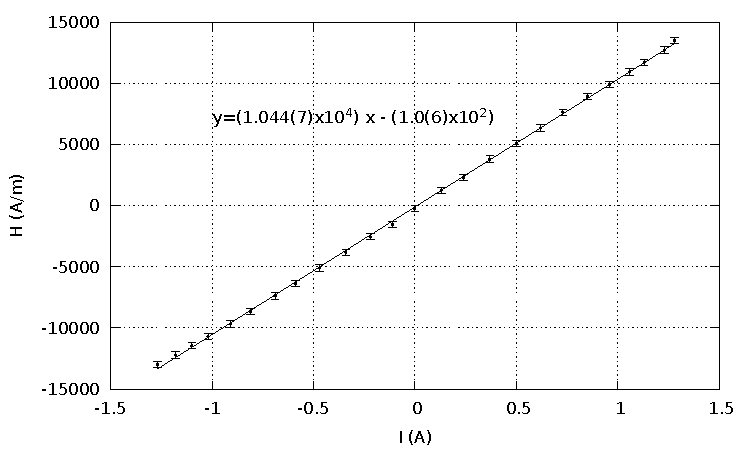
\includegraphics[width=0.7\textwidth]{./Imagens/grafico1.pdf}
\caption{Dados obtidos para o campo $H$ em função da intensidade da corrente $I$, e respectiva regressão linear, efectuada pelo método dos mínimos quadrados.}
\end{figure*}

Seguidamente, realizámos uma regressão linear do tipo $H=\alpha I + \beta $ utilizando os dados representados na Figura 1, pelo método dos mínimos quadrados, e tendo em conta os erros nas duas variáveis pelo método dos erros equivalentes \footnote{No método dos erros equivalentes, para ter em conta ambos os erros, primeiro realiza-se uma regressão linear tendo em conta apenas erros em $y$, a variável dependente. Assim, obtém-se um declive $m$, que é utilizado para calcular um erro total, chamado erro equivalente, dado por $\sigma_{eq}=\sqrt{\sigma_y^2+(m\sigma_x)^2}$. Este erro é então associado novamente à variável dependente, sendo realizada uma nova regressão com este erro, em vez de $\sigma_y$.}. A equação da recta obtida foi:
\begin{equation}
H=(1.044(7)\times 10^{5})~I-(1.0(6)\times 10^{2})
\end{equation}
Tiramos então o valor de $\alpha$ e de $\beta$ e respetivas incertezas $\sigma_{\alpha}$ e $\sigma_{\beta}$ :
$$\alpha \pm \sigma_{\alpha}=(1.044 \pm 0.007) \times 10^{5} \mathrm{~(A/m)}$$
$$\beta \pm \sigma_{\beta}=(-1.0 \pm 0.6) \times 10^{2} \mathrm{~ (m}^{-1})$$
O valor do chi-quadrado reduzido obtido para a regressão linear foi de $ \chi^2=0.28$.

Finalmente, na Figura 2, apresentamos os pontos obtidos para $B$, obtidos pela Equação 2, e para H, obtidos utilizando a recta de calibração obtida.
\begin{figure*}[htbp]
\centering
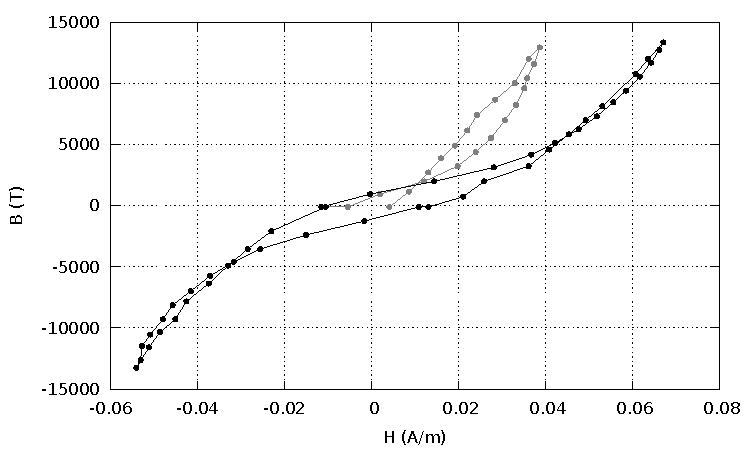
\includegraphics[width=0.7\textwidth]{./Imagens/grafico2.pdf}
\caption{Curva de histerese: campo medido $B$ em função de $H(I)$, determinado pela recta de calibração. A cinzento apresenta-se a primeira parte do ciclo.}
\end{figure*}

\section{Análise e discussão dos dados}

\subsection{Obtençao dos valores do campo magnetico coersivo e remanescente}
Achando as intercepções da curva de histerese obtida com o eixo do $xx$ e $yy$, obtemos respectivamente os valores de $-H_c$ e de $B_r$ que são $-1250.28 (A.m^{-1})$ e $0.013 (T)$

Na equacão da recta de calibracão do solenóide, podemos interpretar o declive como sendo $n$, o número de espiras por unidade de comprimento do solenóide. Sabendo que o solenóide mede sensívelmene 14,5cm e tem 1500 espiras, obtemos $n=10,34\times 10^3$, o que é coerente com o valor expermiental. O valor da ordenada da origem é bastante pequeno, e pode-se atribuir a erros experimentais.

Na figura 2, podemos observar o efeito de histerese do material. Em primeiro lugar, vemos um valor nulo de $H$ a corresponder a um valor nulo de $B$, visto que o material não apresentava magnetização remanescente. No entanto, após se atingir o valor máximo de $H$ aplicado, quando realizamos o processo em sentido inverso, o campo $B$ medido para o mesmo valor de $H$ é superior ao medido quando se realizou este processo pela primeira vez. Isto deve-se ao ``efeito de memória'' que resulta da magnetizacao que o material adquiriu durante o primeiro processo. Isto continua a verificar-se, mas em sentido inverso, uma vez aplicando o máximo de corrente negativa e voltando a descer até $H=0$. Repete-se este processo uma vez mais para valores positivos de corrente, verificando-se de novo a histerese no material.

\newpage
\section{Anexos}
Apresentamos os dados recolhidos da intensidade da corrente na bobine, $I$, e da diferença de potencial $V$ no sensor de Hall para as duas partes da experiência, a calibração e a medida da histerese. Estes dados encontram-se respectivamente nas Tabelas 1 e 2, na forma sugerida. Calculam-se também os campos $B$ e $H$ para cada caso.
\subsection{Dados recolhidos}
\begin{table}[htbp]
\center
\caption{Dados recolhidos de $I$ e $V$ para a calibração; cálculo de $B$ e $H$.}
\begin{tabular}{rlrlrlrl}
\hline
\multicolumn{ 2}{c}{I (A)} & \multicolumn{ 2}{c}{V (V)} & \multicolumn{ 2}{c}{B (G)} & \multicolumn{ 2}{c}{H (A/m)} \\ \hline

0.00 & $\pm$ 0.01 & 2.49 & $\pm$ 0.01 & -3.2 & $\pm$ 3.2 & -2.5$\times 10^{2}$ & $\pm 2.5 \times 10^{2}$  \\ 
0.13 & $\pm$ 0.01 & 2.55 & $\pm$ 0.01 & 16.0 & $\pm$ 3.2 & 1.27$\times 10^{3}$ & $\pm 2.5 \times 10^{2}$  \\ 
0.24 & $\pm$ 0.01 & 2.59 & $\pm$ 0.01 & 28.8 & $\pm$ 3.2 & 2.29$\times 10^{3}$ & $\pm 2.5 \times 10^{2}$  \\ 
0.37 & $\pm$ 0.01 & 2.65 & $\pm$ 0.01 & 48.0 & $\pm$ 3.2 & 3.82$\times 10^{3}$ & $\pm 2.5 \times 10^{2}$  \\ 
0.50 & $\pm$ 0.01 & 2.70 & $\pm$ 0.01 & 64.0 & $\pm$ 3.2 & 5.09$\times 10^{3}$ & $\pm 2.5 \times 10^{2}$  \\ 
0.62 & $\pm$ 0.01 & 2.75 & $\pm$ 0.01 & 80.0 & $\pm$ 3.2 & 6.37$\times 10^{3}$ & $\pm 2.5 \times 10^{2}$  \\ 
0.73 & $\pm$ 0.01 & 2.80 & $\pm$ 0.01 & 96.0 & $\pm$ 3.2 & 7.64$\times 10^{3}$ & $\pm 2.5 \times 10^{2}$  \\ 
0.85 & $\pm$ 0.01 & 2.85 & $\pm$ 0.01 & 112.0 & $\pm$ 3.2 & 8.91$\times 10^{3}$ & $\pm 2.5 \times 10^{2}$  \\ 
0.96 & $\pm$ 0.01 & 2.89 & $\pm$ 0.01 & 124.8 & $\pm$ 3.2 & 9.93$\times 10^{3}$ & $\pm 2.5 \times 10^{2}$  \\ 
1.06 & $\pm$ 0.01 & 2.93 & $\pm$ 0.01 & 137.6 & $\pm$ 3.2 & 1.09$\times 10^{4}$ & $\pm 2.5 \times 10^{2}$  \\ 
1.13 & $\pm$ 0.01 & 2.96 & $\pm$ 0.01 & 147.2 & $\pm$ 3.2 & 1.17$\times 10^{4}$ & $\pm 2.5 \times 10^{2}$  \\ 
1.23 & $\pm$ 0.01 & 3.00 & $\pm$ 0.01 & 160.0 & $\pm$ 3.2 & 1.27$\times 10^{4}$ & $\pm 2.5 \times 10^{2}$  \\ 
1.28 & $\pm$ 0.01 & 3.03 & $\pm$ 0.01 & 169.6 & $\pm$ 3.2 & 1.35$\times 10^{4}$ & $\pm 2.5 \times 10^{2}$  \\ 
-0.11 & $\pm$ 0.01 & 2.44 & $\pm$ 0.01 & -19.2 & $\pm$ 3.2 & -1.53$\times 10^{3}$ & $\pm 2.5 \times 10^{2}$  \\ 
-0.22 & $\pm$ 0.01 & 2.40 & $\pm$ 0.01 & -32.0 & $\pm$ 3.2 & -2.55$\times 10^{3}$ & $\pm 2.5 \times 10^{2}$  \\ 
-0.34 & $\pm$ 0.01 & 2.35 & $\pm$ 0.01 & -48.0 & $\pm$ 3.2 & -3.82$\times 10^{3}$ & $\pm 2.5 \times 10^{2}$  \\ 
-0.47 & $\pm$ 0.01 & 2.30 & $\pm$ 0.01 & -64.0 & $\pm$ 3.2 & -5.09$\times 10^{3}$ & $\pm 2.5 \times 10^{2}$  \\ 
-0.59 & $\pm$ 0.01 & 2.25 & $\pm$ 0.01 & -80.0 & $\pm$ 3.2 & -6.37$\times 10^{3}$ & $\pm 2.5 \times 10^{2}$  \\ 
-0.69 & $\pm$ 0.01 & 2.21 & $\pm$ 0.01 & -92.8 & $\pm$ 3.2 & -7.38$\times 10^{3}$ & $\pm 2.5 \times 10^{2}$  \\ 
-0.81 & $\pm$ 0.01 & 2.16 & $\pm$ 0.01 & -108.8 & $\pm$ 3.2 & -8.66$\times 10^{3}$ & $\pm 2.5 \times 10^{2}$  \\ 
-0.91 & $\pm$ 0.01 & 2.12 & $\pm$ 0.01 & -121.6 & $\pm$ 3.2 & -9.68$\times 10^{3}$ & $\pm 2.5 \times 10^{2}$  \\ 
-1.02 & $\pm$ 0.01 & 2.08 & $\pm$ 0.01 & -134.4 & $\pm$ 3.2 & -1.070$\times 10^{4}$ & $\pm 2.5 \times 10^{2}$  \\ 
-1.10 & $\pm$ 0.01 & 2.05 & $\pm$ 0.01 & -144.0 & $\pm$ 3.2 & -1.146$\times 10^{4}$ & $\pm 2.5 \times 10^{2}$  \\ 
-1.18 & $\pm$ 0.01 & 2.02 & $\pm$ 0.01 & -153.6 & $\pm$ 3.2 & -1.222$\times 10^{4}$ & $\pm 2.5 \times 10^{2}$  \\ 
-1.27 & $\pm$ 0.01 & 1.99 & $\pm$ 0.01 & -163.2 & $\pm$ 3.2 & -1.300$\times 10^{4}$ & $\pm 2.5 \times 10^{2}$  \\ 
\hline
\end{tabular}
\label{calibracao}
\end{table}

\begin{center}
\begin{longtable}[htbp]{rlrlrlrl}
\caption{Dados recolhidos de $I$ e $V$ para a histerese do material; cálculo de $B$ e $G$.} \label{histerese} \\
\hline
\multicolumn{ 2}{c}{I (A)} & \multicolumn{ 2}{c}{V (V)} & \multicolumn{ 2}{c}{B (T)} & \multicolumn{ 2}{c}{H (A/m)} \\ \hline \endfirsthead
\hline
\multicolumn{ 2}{c}{I (A)} & \multicolumn{ 2}{c}{V (V)} & \multicolumn{ 2}{c}{B (T)} & \multicolumn{ 2}{c}{H (A/m)} \\ \hline \endhead
\hline
\multicolumn{8}{c}{(A tabela continua na página seguinte)}
\endfoot
\endlastfoot
0.00 & $\pm$ 0.01 & 2.14 & $\pm$ 0.01 & -115.2 & $\pm$ 3.2 & -1.1$\times 10^{2}$ & $\pm$ 1.2$\times 10^{2}$ \\ 
0.10 & $\pm$ 0.01 & 2.49 & $\pm$ 0.01 & -3.2 & $\pm$ 3.2 & 9.4$\times 10^{2}$ & $\pm$ 1.2$\times 10^{2}$ \\ 
0.20 & $\pm$ 0.01 & 2.95 & $\pm$ 0.01 & 144.0 & $\pm$ 3.2 & 1.99$\times 10^{3}$ & $\pm$ 1.2$\times 10^{2}$ \\ 
0.31 & $\pm$ 0.01 & 3.38 & $\pm$ 0.01 & 281.6 & $\pm$ 3.2 & 3.14$\times 10^{3}$ & $\pm$ 1.2$\times 10^{2}$ \\ 
0.41 & $\pm$ 0.01 & 3.65 & $\pm$ 0.01 & 368.0 & $\pm$ 3.2 & 4.18$\times 10^{3}$ & $\pm$ 1.2$\times 10^{2}$ \\ 
0.50 & $\pm$ 0.01 & 3.82 & $\pm$ 0.01 & 422.4 & $\pm$ 3.2 & 5.12$\times 10^{3}$ & $\pm$ 1.2$\times 10^{2}$ \\ 
0.61 & $\pm$ 0.01 & 3.99 & $\pm$ 0.01 & 476.8 & $\pm$ 3.2 & 6.27$\times 10^{3}$ & $\pm$ 1.3$\times 10^{2}$ \\ 
0.71 & $\pm$ 0.01 & 4.12 & $\pm$ 0.01 & 518.4 & $\pm$ 3.2 & 7.31$\times 10^{3}$ & $\pm$ 1.3$\times 10^{2}$ \\ 
0.82 & $\pm$ 0.01 & 4.24 & $\pm$ 0.01 & 556.8 & $\pm$ 3.2 & 8.46$\times 10^{3}$ & $\pm$ 1.3$\times 10^{2}$ \\ 
0.91 & $\pm$ 0.01 & 4.33 & $\pm$ 0.01 & 585.6 & $\pm$ 3.2 & 9.40$\times 10^{3}$ & $\pm$ 1.3$\times 10^{2}$ \\ 
1.02 & $\pm$ 0.01 & 4.43 & $\pm$ 0.01 & 617.6 & $\pm$ 3.2 & 1.055$\times 10^{4}$ & $\pm$ 1.4$\times 10^{2}$ \\ 
1.13 & $\pm$ 0.01 & 4.51 & $\pm$ 0.01 & 643.2 & $\pm$ 3.2 & 1.170$\times 10^{4}$ & $\pm$ 1.4$\times 10^{2}$ \\ 
1.23 & $\pm$ 0.01 & 4.57 & $\pm$ 0.01 & 662.4 & $\pm$ 3.2 & 1.274$\times 10^{4}$ & $\pm$ 1.4$\times 10^{2}$ \\ 
1.29 & $\pm$ 0.01 & 4.60 & $\pm$ 0.01 & 672.0 & $\pm$ 3.2 & 1.337$\times 10^{4}$ & $\pm$ 1.5$\times 10^{2}$ \\ 
1.16 & $\pm$ 0.01 & 4.49 & $\pm$ 0.01 & 636.8 & $\pm$ 3.2 & 1.201$\times 10^{4}$ & $\pm$ 1.4$\times 10^{2}$ \\ 
1.04 & $\pm$ 0.01 & 4.40 & $\pm$ 0.01 & 608.0 & $\pm$ 3.2 & 1.076$\times 10^{4}$ & $\pm$ 1.4$\times 10^{2}$ \\ 
0.79 & $\pm$ 0.01 & 4.16 & $\pm$ 0.01 & 531.2 & $\pm$ 3.2 & 8.15$\times 10^{3}$ & $\pm$ 1.3$\times 10^{2}$ \\ 
0.68 & $\pm$ 0.01 & 4.04 & $\pm$ 0.01 & 492.8 & $\pm$ 3.2 & 7.00$\times 10^{3}$ & $\pm$ 1.3$\times 10^{2}$ \\ 
0.57 & $\pm$ 0.01 & 3.92 & $\pm$ 0.01 & 454.4 & $\pm$ 3.2 & 5.85$\times 10^{3}$ & $\pm$ 1.2$\times 10^{2}$ \\ 
0.45 & $\pm$ 0.01 & 3.78 & $\pm$ 0.01 & 409.6 & $\pm$ 3.2 & 4.60$\times 10^{3}$ & $\pm$ 1.2$\times 10^{2}$ \\ 
0.32 & $\pm$ 0.01 & 3.63 & $\pm$ 0.01 & 361.6 & $\pm$ 3.2 & 3.24$\times 10^{3}$ & $\pm$ 1.2$\times 10^{2}$ \\ 
0.20 & $\pm$ 0.01 & 3.31 & $\pm$ 0.01 & 259.2 & $\pm$ 3.2 & 1.99$\times 10^{3}$ & $\pm$ 1.2$\times 10^{2}$ \\ 
0.08 & $\pm$ 0.01 & 3.16 & $\pm$ 0.01 & 211.2 & $\pm$ 3.2 & 7.3$\times 10^{2}$ & $\pm$ 1.2$\times 10^{2}$ \\ 
0.00 & $\pm$ 0.01 & 2.91 & $\pm$ 0.01 & 131.2 & $\pm$ 3.2 & -1.0$\times 10^{2}$ & $\pm$ 1.2$\times 10^{2}$ \\ 
0.00 & $\pm$ 0.01 & 2.84 & $\pm$ 0.01 & 108.8 & $\pm$ 3.2 & -1.0$\times 10^{2}$ & $\pm$ 1.2$\times 10^{2}$ \\ 
-0.11 & $\pm$ 0.01 & 2.45 & $\pm$ 0.01 & -16.0 & $\pm$ 3.2 & -1.25$\times 10^{3}$ & $\pm$ 1.2$\times 10^{2}$ \\ 
-0.22 & $\pm$ 0.01 & 2.03 & $\pm$ 0.01 & -150.4 & $\pm$ 3.2 & -2.40$\times 10^{3}$ & $\pm$ 1.2$\times 10^{2}$ \\ 
-0.33 & $\pm$ 0.01 & 1.70 & $\pm$ 0.01 & -256.0 & $\pm$ 3.2 & -3.55$\times 10^{3}$ & $\pm$ 1.2$\times 10^{2}$ \\ 
-0.43 & $\pm$ 0.01 & 1.51 & $\pm$ 0.01 & -316.8 & $\pm$ 3.2 & -4.59$\times 10^{3}$ & $\pm$ 1.2$\times 10^{2}$ \\ 
-0.54 & $\pm$ 0.01 & 1.34 & $\pm$ 0.01 & -371.2 & $\pm$ 3.2 & -5.74$\times 10^{3}$ & $\pm$ 1.2$\times 10^{2}$ \\ 
-0.66 & $\pm$ 0.01 & 1.20 & $\pm$ 0.01 & -416.0 & $\pm$ 3.2 & -6.99$\times 10^{3}$ & $\pm$ 1.3$\times 10^{2}$ \\ 
-0.77 & $\pm$ 0.01 & 1.07 & $\pm$ 0.01 & -457.6 & $\pm$ 3.2 & -8.14$\times 10^{3}$ & $\pm$ 1.3$\times 10^{2}$ \\ 
-0.88 & $\pm$ 0.01 & 1.00 & $\pm$ 0.01 & -480.0 & $\pm$ 3.2 & -9.29$\times 10^{3}$ & $\pm$ 1.3$\times 10^{2}$ \\ 
-1.00 & $\pm$ 0.01 & 0.91 & $\pm$ 0.01 & -508.8 & $\pm$ 3.2 & -1.054$\times 10^{4}$ & $\pm$ 1.4$\times 10^{2}$ \\ 
-1.09 & $\pm$ 0.01 & 0.85 & $\pm$ 0.01 & -528.0 & $\pm$ 3.2 & -1.148$\times 10^{4}$ & $\pm$ 1.4$\times 10^{2}$ \\ 
-1.20 & $\pm$ 0.01 & 0.84 & $\pm$ 0.01 & -531.2 & $\pm$ 3.2 & -1.263$\times 10^{4}$ & $\pm$ 1.4$\times 10^{2}$ \\ 
-1.26 & $\pm$ 0.01 & 0.81 & $\pm$ 0.01 & -540.8 & $\pm$ 3.2 & -1.326$\times 10^{4}$ & $\pm$ 1.5$\times 10^{2}$ \\ 
-1.10 & $\pm$ 0.01 & 0.90 & $\pm$ 0.01 & -512.0 & $\pm$ 3.2 & -1.159$\times 10^{4}$ & $\pm$ 1.4$\times 10^{2}$ \\ 
-0.98 & $\pm$ 0.01 & 0.98 & $\pm$ 0.01 & -486.4 & $\pm$ 3.2 & -1.033$\times 10^{4}$ & $\pm$ 1.4$\times 10^{2}$ \\ 
-0.88 & $\pm$ 0.01 & 1.09 & $\pm$ 0.01 & -451.2 & $\pm$ 3.2 & -9.29$\times 10^{3}$ & $\pm$ 1.3$\times 10^{2}$ \\ 
-0.74 & $\pm$ 0.01 & 1.17 & $\pm$ 0.01 & -425.6 & $\pm$ 3.2 & -7.83$\times 10^{3}$ & $\pm$ 1.3$\times 10^{2}$ \\ 
-0.60 & $\pm$ 0.01 & 1.33 & $\pm$ 0.01 & -374.4 & $\pm$ 3.2 & -6.37$\times 10^{3}$ & $\pm$ 1.2$\times 10^{2}$ \\ 
-0.46 & $\pm$ 0.01 & 1.47 & $\pm$ 0.01 & -329.6 & $\pm$ 3.2 & -4.90$\times 10^{3}$ & $\pm$ 1.2$\times 10^{2}$ \\ 
-0.33 & $\pm$ 0.01 & 1.61 & $\pm$ 0.01 & -284.8 & $\pm$ 3.2 & -3.55$\times 10^{3}$ & $\pm$ 1.2$\times 10^{2}$ \\ 
-0.19 & $\pm$ 0.01 & 1.78 & $\pm$ 0.01 & -230.4 & $\pm$ 3.2 & -2.09$\times 10^{3}$ & $\pm$ 1.2$\times 10^{2}$ \\ 
0.00 & $\pm$ 0.01 & 2.17 & $\pm$ 0.01 & -105.6 & $\pm$ 3.2 & -1.0$\times 10^{2}$ & $\pm$ 1.2$\times 10^{2}$ \\ 
0.00 & $\pm$ 0.01 & 2.33 & $\pm$ 0.01 & -54.4 & $\pm$ 3.2 & -1.0$\times 10^{2}$ & $\pm$ 1.2$\times 10^{2}$ \\ 
0.10 & $\pm$ 0.01 & 2.56 & $\pm$ 0.01 & 19.2 & $\pm$ 3.2 & 9.4$\times 10^{2}$ & $\pm$ 1.2$\times 10^{2}$ \\ 
0.20 & $\pm$ 0.01 & 2.88 & $\pm$ 0.01 & 121.6 & $\pm$ 3.2 & 1.99$\times 10^{3}$ & $\pm$ 1.2$\times 10^{2}$ \\ 
0.32 & $\pm$ 0.01 & 3.12 & $\pm$ 0.01 & 198.4 & $\pm$ 3.2 & 3.24$\times 10^{3}$ & $\pm$ 1.2$\times 10^{2}$ \\ 
0.43 & $\pm$ 0.01 & 3.25 & $\pm$ 0.01 & 240.0 & $\pm$ 3.2 & 4.39$\times 10^{3}$ & $\pm$ 1.2$\times 10^{2}$ \\ 
0.54 & $\pm$ 0.01 & 3.36 & $\pm$ 0.01 & 275.2 & $\pm$ 3.2 & 5.54$\times 10^{3}$ & $\pm$ 1.2$\times 10^{2}$ \\ 
0.68 & $\pm$ 0.01 & 3.46 & $\pm$ 0.01 & 307.2 & $\pm$ 3.2 & 7.00$\times 10^{3}$ & $\pm$ 1.3$\times 10^{2}$ \\ 
0.80 & $\pm$ 0.01 & 3.54 & $\pm$ 0.01 & 332.8 & $\pm$ 3.2 & 8.25$\times 10^{3}$ & $\pm$ 1.3$\times 10^{2}$ \\ 
0.93 & $\pm$ 0.01 & 3.60 & $\pm$ 0.01 & 352.0 & $\pm$ 3.2 & 9.61$\times 10^{3}$ & $\pm$ 1.3$\times 10^{2}$ \\ 
1.01 & $\pm$ 0.01 & 3.62 & $\pm$ 0.01 & 358.4 & $\pm$ 3.2 & 1.044$\times 10^{4}$ & $\pm$ 1.4$\times 10^{2}$ \\ 
1.12 & $\pm$ 0.01 & 3.67 & $\pm$ 0.01 & 374.4 & $\pm$ 3.2 & 1.159$\times 10^{4}$ & $\pm$ 1.4$\times 10^{2}$ \\ 
1.25 & $\pm$ 0.01 & 3.71 & $\pm$ 0.01 & 387.2 & $\pm$ 3.2 & 1.295$\times 10^{4}$ & $\pm$ 1.5$\times 10^{2}$ \\ 
1.16 & $\pm$ 0.01 & 3.63 & $\pm$ 0.01 & 361.6 & $\pm$ 3.2 & 1.201$\times 10^{4}$ & $\pm$ 1.4$\times 10^{2}$ \\ 
0.97 & $\pm$ 0.01 & 3.53 & $\pm$ 0.01 & 329.6 & $\pm$ 3.2 & 1.003$\times 10^{4}$ & $\pm$ 1.4$\times 10^{2}$ \\ 
0.84 & $\pm$ 0.01 & 3.39 & $\pm$ 0.01 & 284.8 & $\pm$ 3.2 & 8.67$\times 10^{3}$ & $\pm$ 1.3$\times 10^{2}$ \\ 
0.72 & $\pm$ 0.01 & 3.26 & $\pm$ 0.01 & 243.2 & $\pm$ 3.2 & 7.42$\times 10^{3}$ & $\pm$ 1.3$\times 10^{2}$ \\ 
0.60 & $\pm$ 0.01 & 3.19 & $\pm$ 0.01 & 220.8 & $\pm$ 3.2 & 6.16$\times 10^{3}$ & $\pm$ 1.2$\times 10^{2}$ \\ 
0.48 & $\pm$ 0.01 & 3.10 & $\pm$ 0.01 & 192.0 & $\pm$ 3.2 & 4.91$\times 10^{3}$ & $\pm$ 1.2$\times 10^{2}$ \\ 
0.38 & $\pm$ 0.01 & 3.00 & $\pm$ 0.01 & 160.0 & $\pm$ 3.2 & 3.87$\times 10^{3}$ & $\pm$ 1.2$\times 10^{2}$ \\ 
0.27 & $\pm$ 0.01 & 2.91 & $\pm$ 0.01 & 131.2 & $\pm$ 3.2 & 2.72$\times 10^{3}$ & $\pm$ 1.2$\times 10^{2}$ \\ 
0.12 & $\pm$ 0.01 & 2.77 & $\pm$ 0.01 & 86.4 & $\pm$ 3.2 & 1.15$\times 10^{3}$ & $\pm$ 1.2$\times 10^{2}$ \\ 
0.00 & $\pm$ 0.01 & 2.63 & $\pm$ 0.01 & 41.6 & $\pm$ 3.2 & -1.0$\times 10^{2}$ & $\pm$ 1.2$\times 10^{2}$ \\
\hline
\end{longtable}
\end{center}
\newpage
\subsection{Cálculo dos erros associados às medidas}
Na secção 3, as grandezas obtidas foram medidas directamente, pelo que os erros foram estimados tendo em conta o método de medição usado. No entanto, na secção 4, as grandezas foram calculadas a partir das obtidas directamente, pelo que há propagações de erros envolvidas. Esses erros foram calculados pela fórmula de propagação de erros: \begin{equation} \delta f(x_1,x_2,\ldots,x_n)=\sqrt{\sum_{i=1}^{n}\left( \frac{\partial f}{\partial x_i}\delta x_i \right)^2}\end{equation}.

Aqui, $f$ é uma grandeza calculada a partir das grandezas $x_1,x_2,\ldots,x_n$, e $\delta x_i$ são os erros associados às mesmas. Na Tabela 4 apresentamos as equações das grandezas calculadas bem como os respetivos erros.
\renewcommand{\arraystretch}{2.5}
\begin{table}[htbp]
\begin{center}
\caption{Resumo das equações utilizadas para efectuar o cálculo de grandezas relevantes e o respectivo erro, calculado pela fórmula de propagação de erros - equação (4).}
\begin{tabular}{lll}
\textbf{Grandeza} & $f(x_1,x_2,\ldots,x_n)$ & $\delta f(x_1,x_2,\ldots,x_n)$ \\ \hline
\textbf{Área}&$\displaystyle A=\pi\left(\frac{d}{2}\right)^2 $ & $\displaystyle \delta A= \frac{\pi d}{2}\delta d $ \\
\textbf{Área média} &$\displaystyle A_g=\frac{A_i+A_f}{2}$ & $ \displaystyle\delta A_g=\frac{1}{2}\sqrt{\delta A_i^2+\delta A_f^2}$ \\
\textbf{Taxa de fusão} &$\displaystyle R=R_a=\frac{m_f-m_i}{\Delta t}$&$ \displaystyle\delta R=\delta R_a= \sqrt{\left( \frac{\delta m_i}{\Delta t}\right)^2+\left( \frac{m_f}{\Delta t}\right)^2+\left( \frac{m_f-m_i}{\Delta t^2}\delta(\Delta t)\right)^2}$ \\
\textbf{Taxa de fusão efectiva}&$\displaystyle R_0=R-R_a$ & $ \displaystyle \delta R_0= \sqrt{\delta R^2+\delta R_a^2}$ \\
\textbf{Condutividade}&$\displaystyle k=\frac{R_0 L_g h}{A_g \Delta T} $& $ \displaystyle \delta k= k\sqrt{\left(\frac{\delta R_0}{R_0}\right)^2+\left(\frac{\delta h}{h}\right)^2+\left(\frac{\delta A_g}{A_g}\right)^2}$ \\ [2ex] \hline
\end{tabular}
\end{center}
\end{table}

\end{document}